\documentclass{article}
\usepackage[utf8]{inputenc}
\usepackage{kpfonts}
\usepackage{commath}
\usepackage{amsthm}
\usepackage{graphicx}
\usepackage[margin=0.8in]{geometry}

\newcommand{\R}{\ensuremath{\mathbb{R}}}
\newcommand{\N}{\ensuremath{\mathbb{N}}}
\newcommand{\closure}[1]{\ensuremath{\Bar{#1}}}
\newcommand{\oBall}[3][\empty]{\ensuremath{B^{#1}_{#2}(#3)}}
\newcommand{\fRR}{\ensuremath{f:\R \to \R}}
\newcommand{\define}[1]{\textbf{\underline{#1}}}
\newcommand{\ts}{\text topological space}
\newcommand{\tp}{\ensuremath{\mathcal{T}}}
\newcommand{\es}{\ensuremath{\emptyset}}
\newcommand{\tpcof}{\ensuremath{\tp_\text{cof}}}
\newcommand{\tpdisc}{\ensuremath{\tp_\text{disc}}}
\newcommand{\tptriv}{\ensuremath{\tp_\text{triv}}}
\newcommand{\union}{\cup}
\newcommand{\Union}{\bigcup}
\newcommand{\inter}{\cap}
\newcommand{\Inter}{\bigcap}
\renewcommand{\Subset}{\subseteq}
\renewcommand{\Supset}{\supseteq}

\theoremstyle{definition}
\newtheorem*{definition}{Definition}
\newtheorem*{theorem}{Theorem}

\theoremstyle{remark}
\newtheorem*{remark}{Remark}

\begin{document}
    \begin{center}
        \textsc{Dillan Marroquin\\MATH 440.1001\\Scribing Week 3\\Due. 15 February 2021\\}
    \end{center}
    \begin{center}
        \underline{\textsc{MATH 440 Problems}}
    \end{center}
    
    \subsection*{Review of Last Lecture}
        The closed subsets in $(X, \tpcof)$ are $X$ and all finite subsets of $X$.\\
        If $X$ is a finite set, then $\tpcof = \tpdisc$.
    \noindent\section*{\textbf{\textsc{Lecture 7}}}
        \begin{definition}[7.1]
        Let $(X,\tp)$ be a topological space and let $A \Subset X$ be a subset. Let $\tp_A := \{U \inter A | U \in \tp\}$. Then $(A, \tp_A)$ is a topological space and $\tp$ is called the \define{subspace topology} on $A$.
        \end{definition}
        
        \noindent Definition 7.1 gives many interesting examples of spaces:
        \begin{enumerate}
            \item Graph $(\fRR) \Subset \R^2$, i.e. the Euclidean Topology.
            \item $S^2 := \{(x,y,z) | x^2+y^2+z^2 = 1\}$, i.e. the "2-sphere."\\
            \begin{center}
                \graphicspath{images}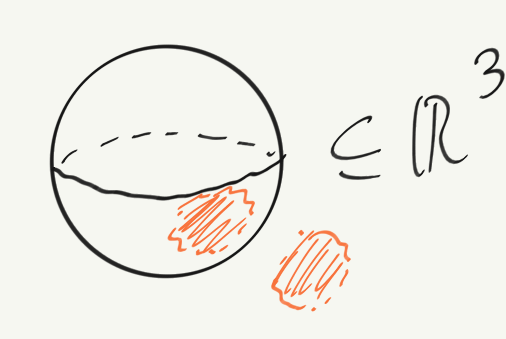
\includegraphics[scale = 0.25]{images/Sphere.png}
            \end{center}
            \item Knots in $\R^3$.
            \item The Order topology.
            \item Lower/Upper Limit topology on $\R$.
            \item \ldots and others.
        \end{enumerate}
        
    \section*{\textbf{\textsc{Lecture 8}}
        \subsection*{Closed Sets/Limit Points in Topological Spaces}}
            \begin{theorem}[8.1]
                Let $X$ be a \ts. Then:
                \begin{enumerate}
                    \item $X, \es$ are closed subsets.
                    \item Finite unions of closed subsets are closed.
                    \item Arbitrary intersections of closed subsets are closed.
                \end{enumerate}
            \end{theorem}
        \noindent The proof of Theorem 8.1 is a direct consequence of applying DeMorgan's Laws to Definition 6.1.\\
        Recall Definition 4.1 of closed subsets in Euclidean space:
        \begin{definition}[4.1]
            Let $A \Subset \R^n$ be a subset. Then $A$ is \define{closed} iff every convergent sequence $\{a_k\} \Subset A$ converges in $A$, i.e. $\lim\limits_{k \to \infty} a_k \in A$.
        \end{definition}
        \noindent We will use this definition to help us understand the following definition:
        \begin{definition}[8.2]
            Let $X$ be a \ts{} where $A \Subset X$ is a subset. A point $y \in X$ is a \define{limit point} of $A$ iff $\forall$ open subsets $U \Subset X$ containing $y$, $A \inter (U-\{y\}) \neq \es$.\\
            We will define $L(A) := \{y \in X | \text{$y$ is a limit point of $A$}\} := A'$
        \end{definition}
        
        \subsection*{Examples in $\R^1$}
            \begin{enumerate}
                \item Define $A := (0,1]$.
                \begin{enumerate}
                    \item Show $0 \in L(A)$.\\
                    Let $U \Subset \R$ be an open subset such that $0 \in U$. Then $\exists\varepsilon > 0$ such that $\oBall{0}{\varepsilon} = (-\varepsilon, \varepsilon) \Subset U$. Therefore $U - \{0\} \Supset (0, \varepsilon) \implies U-\{0\} \inter A \neq \es$.
                    \item Show $1 \in L(A)$.\\
                    Let $U \Subset \R$ be an open subset such that $1 \in U$. Then $\exists\varepsilon > 0$ such that $\oBall{1}{\varepsilon} \Subset U$. Then $U - \{1\} \Supset (1-\varepsilon, 1) \implies U-\{1\} \inter A \neq \es$.
                    \item We can apply this same strategy to prove that $L(A) = [0,1]$.
                \end{enumerate}
                \item Let $A = \{\frac{1}{n} | n \in \N\}$.\\
                It is obvious that since $\frac{1}{n} \to 0$, then $0 \in L(A)$.\\
                If $x \neq 0$ and $x \in L(A)$, then $\exists$ a subsequence of $\{\frac{1}{n}\}_{n \geq 0} \to x \neq 0$. This is a contradiction since every convergent subsequence of $\{\frac{1}{n}\}$ converges to $0$.\\
                In particular, $\forall \frac{1}{n} \in A, \exists$ and open subset $U \Supset \frac{1}{n}$ such that $A \inter U = \{\frac{1}{n}\}$.
            \end{enumerate}
            \begin{theorem}[8.4]
                Let $X$ be a \ts{} and let $A \Subset X$ be a subset. Then $A$ is \define{closed} iff $L(A) \Subset A$.
            \end{theorem}
        
    \section*{\textbf{\textsc{Lecture 9}}}
    \begin{remark}[8.4]
        Recall Theorem 8.4 from last lecture. This is a useful trick to show that a subset $V \Subset X$ is open. $\forall y \in V$, find an open subset $U_y \Subset X$ such that $y \in U_y$ and $U_y \Subset V$. Then
            \begin{align*}
                &\implies V = \Union_{y \in V} U_y     \qquad\textit{By Axiom 2 of \ts{}}\\
                &\implies \text{V is open.}
            \end{align*}
    \end{remark}
    
    \begin{definition}[9.2]
        Let $X$ be a \ts{} and $A \Subset X$ a subset. Then the \define{closure} of $A$ in $X$, $\closure{A}$, is the intersection of all closed subsets of $X$ containing $A$:
            \[\closure{A} := \Inter_{B \Subset \text{$X$ closed, $A \Subset B$}}B\]
    \end{definition}
    
    \begin{remark}[9.2] There are a few remarks:
        \begin{enumerate}
            \item \closure{A} is closed by \#3 in Theorem 8.1.
            \item If $B$ is closed and $A \Subset B$, then $A \Subset \closure{A} \Subset B$. Hence $\closure{A}$ is the "smallest" closed subset of $X$ that contains $A$.
            \item If $A$ is closed, then $\closure{A} = A$.
        \end{enumerate}
    \end{remark}

    \subsection*{Intuitive Examples of Closure}
        \begin{enumerate}
            \item $A = (0,1), \, X = \R$.\\
            Then $\closure{A} = [0,1] \Subset [-\frac{1}{n}, 1+\frac{1}{n}], \, \forall n \in \N \implies \closure{A} \Subset \Inter_{n \in \N} [-\frac{1}{n}, 1+\frac{1}{n}]$.
            \item $A = \oBall{\Vec{0}}{\varepsilon}, \, X=\R^2$.\\
            Then
            \begin{center}
                \graphicspath{images}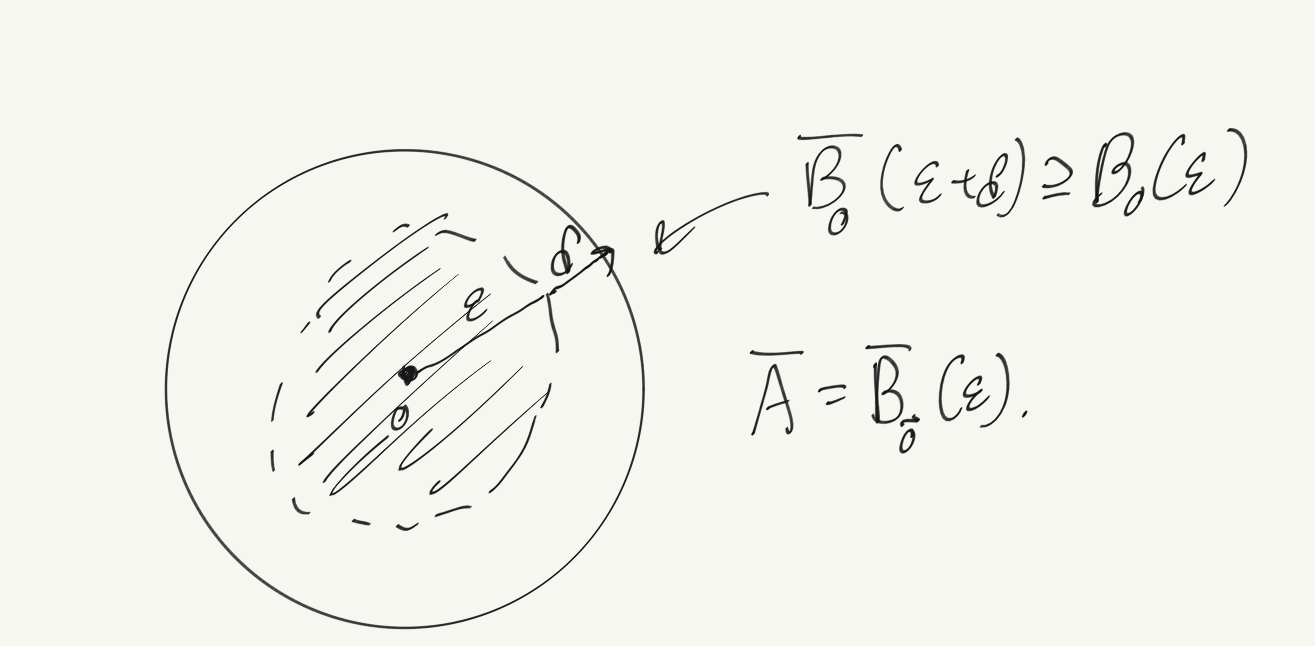
\includegraphics[scale = 0.2]{images/Open Ball.png}
            \end{center}
            \item $A = (0,1), \, X=(\R, \tpdisc)$.\\
            Then $\closure{A} = A$ since $A$ is already closed.
            \item $A = (0,1), \, X=(\R, \tptriv)$.\\
            Then $\closure{A} = \R$.
        \end{enumerate}
        
        \begin{theorem}[9.5]
            Let $A \Subset X$ be a subset of the \ts{} $X$. Then $\closure{A} = A \union L(A)$.
        \end{theorem}
\end{document}